%\documentclass[preprint]{aastex}
\documentclass{emulateapj}
%\documentclass{article}
\usepackage{graphicx}
\usepackage{natbib}
%\bibliographystyle{apj}
\usepackage{amssymb}
\usepackage{amsmath}
\usepackage{float}


\def\h{H$^-$}
\def\chii{$\chi$}
\def\beq{\begin{equation}}
\def\eeq{\end{equation}}
\def\texrm{\textrm}

\interfootnotelinepenalty=9500

\begin{document}

\title{\h\ Opacity in the Solar Atmosphere}

\author{Joshua Wallace}

\affil{AST 514, Department of Astrophysical Sciences, Princeton
  University, Princeton, NJ 08544}

\begin{abstract}
A review of H$^-$ in stellar atmospheres. \h\ provides the dominant
contribution to photospheric opacity in the sun for visible and
near-infrared wavelengths and a significant contribution for
near-ultraviolet wavelengths through both bound-free and free-free absorption.  The dominance of \h\ opacity at these
wavelengths is not a ubiquitous feature of all stars but is sensitive
to \h\ abundance, which is in turn affected by photospheric
temperature and the presence of free electron donors in the form of
low ionization potential metals.  The Saha ionization equation is used
to calculate the relative contributions of various atoms to the
electron number density in the solar photosphere, with alkali and alkaline earth metals shown
to be the dominant contributors.  The fraction of \h\ to H is
calculated and compared with H Paschen abundances to explain why
\h\ provides the dominant contribution to opacity in the optical.
The free-free absorption contribution in the near-infrared is also
discussed with special attention paid to the free-free/bound-free
turnover in dominant opacity contribution source.  A brief look at
\h\ in other astrophysical contexts.
\end{abstract}

\keywords{Sun: atmosphere --- stars: atmospheres}

\section{Introduction}

The \h\ ion has long been recognized as an important source of
continuum opacity in the sun at visible
wavelengths. \citet{Wildt1939a,Wildt1939b} was among the first to
recognize this.  The \h\ ion is, quite simply, a hydrogen atom with an extra electron.  This extra electron
has a relatively low ionization potential of $\chi = 0.754$ eV
(\citealt{carroll2007introduction}, which corresponds to a photon
wavelength of $\sim 16500$\AA.  It is, in part, due to this low
ionization potential that \h\ provides such  a significant contribution to the opacity of the sun's
photosphere in the visible and near-infrared.  \h\ opacities are relevant in all
stars cooler than F0 (\citealt{carroll2007introduction}). \h\
abundance (and therefore its contribution to the opacity) is sensitive 
to temperature and to the abundance of low-\chii\ metals
(\citealt{hansen1994stellar}), primarily the alkali and alkaline earth metals.  The temperature dependence of \h\
abundance can be characterized qualitatively as follows: the gas needs
to be of high enough temperature to allow free electrons (ionized from
low-\chii\ metals as well as some hydrogen) to exist.  The gas,
however, also needs to be of low enough temperature that the
lightly-bound second electrons are not quickly stripped from the
hydrogen atoms either through collisional ionization or a large flux
of photons.  Thus, if the temperature is too low \h\ ions will not be
produced and if the temperature is too high \h\ ions won't survive
long enough to make significant contributions to the opacity.

As far as a qualitative picture for opacity dependence on metallicity,
well, that's where figure 4.4 comes in.

Note to Joshua:  \cite{hansen1994stellar} figure 4.4 provides a figure
of \h\ opacities, I think the temperature dependence.


%\section{Brief History of the Development of the Understanding of \h's Importance in the Sun}
%The existence of \h\ was proven by \cite{bethe1929}.  %He used a three-parameter wavefunction of the form $(1+\alpha
Its astrophysical importance was recognized by \citet{Wildt1939a,Wildt1939b}.


\section{The Nature of the \h\ Ion}
The non-relativistic, Coulomb-interaction Hamiltonian for \h\ is given by 
\begin{equation}
\label{eq:H}
H = \frac{p_1^2}{2m_e} + \frac{p_2^2}{2m_e} - \frac{1}{4\pi\epsilon_0}\frac{e^2}{r_1} -  \frac{1}{4\pi\epsilon_0}\frac{e^2}{r_2} +  \frac{1}{4\pi\epsilon_0}\frac{e^2}{r_{12}}
\eeq
where $m_e$ is the mass of the electron, $p$ is the classical kinetic energy of the electron specified by the subscript, $e$ is the charge of the electron, $\epsilon_0$ is the vacuum permittivity, $r_1$ is the distance from the first electron to the nucleus, $r_2$ is the corresponding value for the second electron, and $r_{12}$ is the distance between the two electrons.  In this Hamiltonian the nucleus is assumed to be fixed.  This Hamiltonian possesses a term for each electron's kinetic energy, each electron's potential energy from its interaction with the nucleus (a single proton), and (specifically the last term in equation~\ref{eq:H}) a term for the repulsive Coulomb interaction between the two electrons.

Many approaches have been taken to calculate wavefunctions for \h.
Many-paramter Hylleraas functions are among the most commonly used.  I will focus on a simple two-parameter trial wavefunction used by \cite{chandra1944} because of the interpretations to which the simple wavefunction lends itself.  The wavefunction is
\beq
\label{eq:chandra}
\psi = \exp(-\alpha r_1 - \beta r_2) + \exp(-\alpha r_2 - \beta r_1).
\eeq
Chandrasekhar showed that the minimum energy of this wavefunction
($E_1=-0.51330$ at $\alpha = 1.03925$ and $\beta = 0.28309$) is
sufficient to provide binding for \h.  The wavefunction gives the
electrons a radial hierarchy, with one electron in close to the
nucleus and the other far away from the nucleus (which gives it its
correspondingly smaller binding energy). Chandrasekhar then, in the
same work, builds on the trial wavefunction in equation~\ref{eq:chandra} by
adding a term that accounts for the fact that one electron is
signficantly screened from the nucleus while the other electron is
practically unscreened, giving a trial wavefunction of the form
\beq
\label{eq:chandra2}
\psi = \left( e^{(-\alpha r_1 - \beta r_2)} + e^{(-\alpha r_2 - \beta r_1)} \right)
\times (1 + c r_{12}).
\eeq
% Additionally, the innermost electron
The energy is minimized with the values $a=1.07478,~b=0.47758,$ and
$c=0.31214$, giving an energy of $E_2=-0.52592$.  Chandrasekhar then
remarks that the addition of this term reduces the screening of the
outer electron (as can be seen by the fact that $E_2 < E_1$, showing
that the outermost electron is more bound in
equation~\ref{eq:chandra2} than in equation~\ref{eq:chandra}).  He
attributes this to the strong polarizability of the hydrogen atom (it
being just a single positive and a single negative charge, thus always
possesing a strong dipole component in the electric field).  A
classical picture of the \h\ ion is shown in
figure~\ref{fig:classical}. The radial hierarchy is seen, with a clear
inner and a clear outer electron.  This cartoon also provides a visual explanation of how the polarization of the H atom's electric field allows a second electron to bind: by positioning themselves opposite the nucleus from each other each electron is able to maximize its own Coulomb attraction to the nucleus in the presence of the other electron.
\begin{figure}
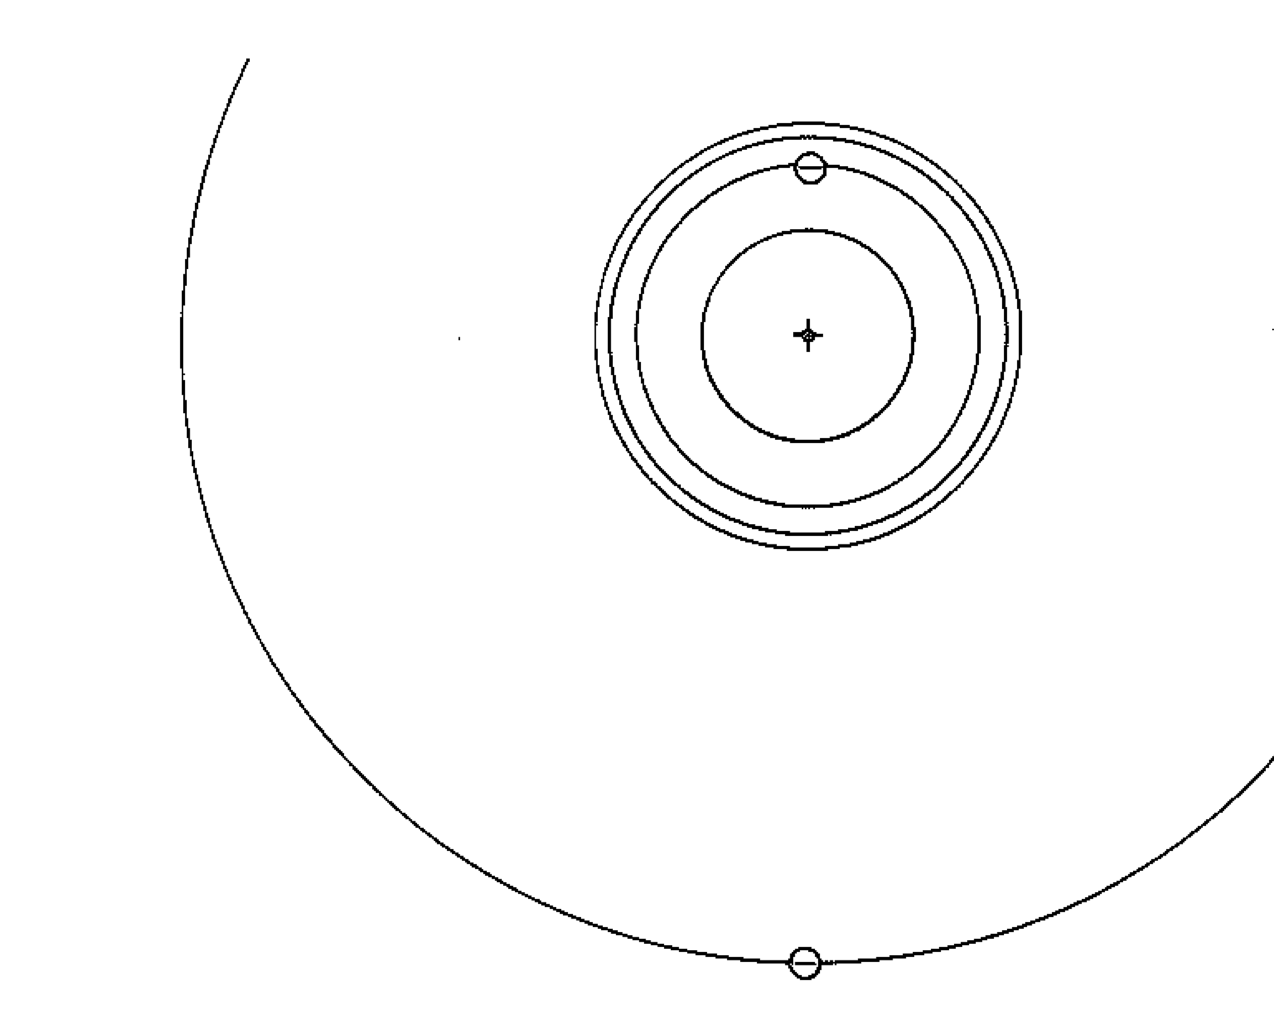
\includegraphics[width=\linewidth]{figs/classicalbohr.png}
\caption{\label{fig:classical}From \cite{collins1989}. A classical Bohr hydrogen atom with an additional electron bound to form an \h\ ion.}
\end{figure}

It has been rigorously shown that \h\ has no bound excited states,
i.e., the only bound state is the ground state (\citealt{hill1977}).
As such, \h\ does not have a line spectrum; there are no electronic transitions between bound states that absorb and emit photons of specific wavelengths.  Its main contribution to the opacity of the solar atmosphere is through continuum absorption of photons with energy greater than the binding energy of its least bound electron.  

The effect screening due to free electrons has on the binding energy of the \h\ ion has been looked at.  The partially ionized nature of the solar atmosphere makes this a relevant study.  \cite{phelpsbajaj1983} use a variational approach to show that the effect screening due to free electrons has on the binding energy of the \h\ ion is within a factor of 2 (as they quantify it) of the effect of screening on the binding energy of a single-electron H atom, despite the electron of the neutral H being $\sim 18$ times more bound than the least bound electron of \h.  To be specific, \cite{phelpsbajaj1983} 
%define a screening parameter $\delta$, where
%\beq
%\delta^2 = \sum_i \frac{4\pi n e^2}{k_B T}\left[ \frac{F_{-1/2}(\nu_i)}{F_{1/2}(\nu_i)}
%\eeq
assume a Dingle-Mansfield screening, which modifies equation~\ref{eq:H} to
\beq
H = \frac{p_1^2 + p_2^2}{2m_e} - \frac{1}{4\pi\epsilon_0}\frac{e^2}{r_1}e^{-\delta r_1} -  \frac{1}{4\pi\epsilon_0}\frac{e^2}{r_2}e^{-\delta r_2} + \\
 \frac{1}{4\pi\epsilon_0}\frac{e^2}{r_{12}} e^{-\delta r_{12}}
\eeq
where $\delta$ is a screening parameter defined in the text.  For my
purpose of comparison the exact definition of the screening parameter
is not necessary to include.  Their results are shown in
figure~\ref{fig:screening}.  They calculate that for  \h\ the binding
energy goes to zero for $a_0 \delta = 0.87$  (where $a_0$ is the Bohr
radius) while it is shown elsewhere that for H binding energy goes to
zero for $a_0 \delta = 1.2$ (\citealt{rogersetal1970}).  The two
values of $a_0 \delta$ are not very different which, as mentioned
previous, seems surprising due to the factor $~18$ discrepancy between
the binding energies of H and \h.  \cite{phelpsbajaj1983} attribute
this to the assumption that the interactions between the proton and
the electrons and the interaction between the electrons themselves are
modified in the presence of free electrons and so the ground state
energy is itself modified as a function of $\delta$; the binding
energy is modified by both the presence of free electrons and by the change in the ground state energy in the presence of free electrons.  The interplay of these two effects is what allows a perhaps intially surprisingly large value of $a_0 \delta$ for the binding energy to go to zero in \h.
\begin{figure}
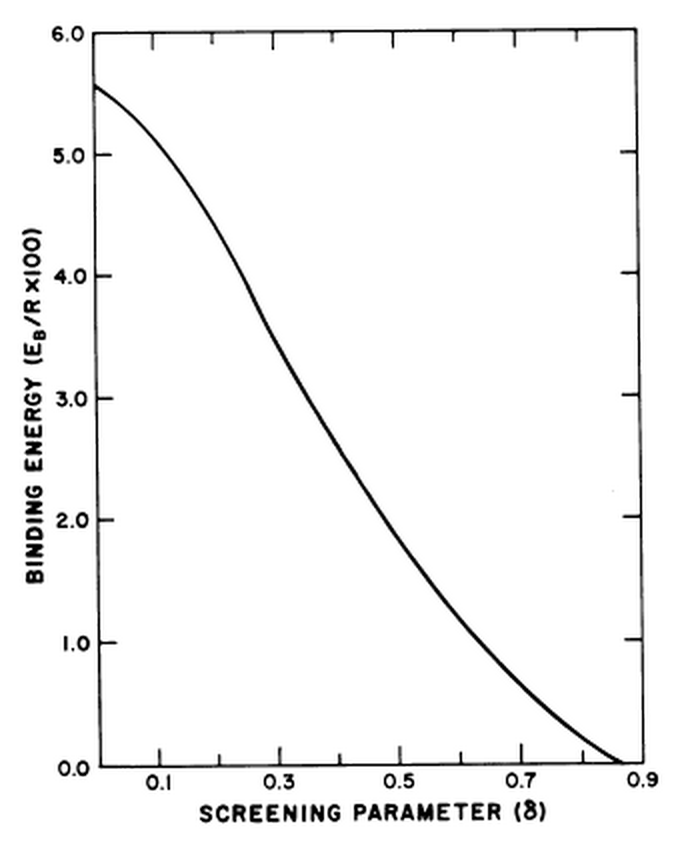
\includegraphics[width=76mm]{figs/screeningparameter.png}%normal width
                                %is 80mm
\caption{\label{fig:screening}From \cite{phelpsbajaj1983}. Binding energy of the least bound
electron in the \h\ ion as a function of screening parameter
$\delta$.  Binding energy is given in units of the Rydberg energy and
multiplied by 100.}
\end{figure}

To show the impact this screening has on \h\ opacity in the sun I will
reference figure~\ref{fig:screeninge}, taken from \cite{phelpsbajaj1983}.
The sun's photospheric temperature lies between the two temperature
curves of $4000K$ and $8000K$.  Simple order of magnitude arguments
will allow us to see that $\delta$ is small for the solar photosphere
without actually having to know the value for electron number
density.  The density of the photosphere is $\sim 1$ g/cm$^{-3}$, so
 there are Avogadro's number of electrons per cm$^{-3}$ in the
 photosphere, providing an upper limit of $\delta\sim 1$ based on
 figure~\ref{fig:screeninge}.  However, most electrons are still bound to
 their atoms in the photosphere.  \cite{boehm1989} calculates that
 the ionization fraction of H in the solar photosphere is $10^-4$.  H
 is the majority consituent of the solar photosphere; the next major
 constituent, He, has too large an ionization potential to be
 significantly ionized at these temperatures.  The metals of the
 photosphere have varying abundances and ionization states so it is
 less straightforward to calculate an ionization fraction for the
 metals, but since they only make up $\sim$1\%\ of the solar
 photosphere as long as their ionization fraction is less than
 $10^{-3}$ the metallic contribution will be comparable to that of H.
 This seems to be reasonable as an upper limit to the ionization
 fraction of metals, because, although some metals have lower
 ionization potentials than H, others have larger ionization
 potentials.  Additionally, ionization potential increases fairly
 sharply as a function of degree of ionization of an ion, so there is
 a low probability that metals will contribute more than one electron
 per atom/ion, for those species that do actually ionize.  With these
 arguments I set an upper limit on the free electron number density at
 $\sim 10^{19}$, which is $\sim 10^{-4} \times$ Avogadro's number.
 This gives a $\delta$ slightly larger than $10^{-2}$, which,
 referencing figure~\ref{fig:screening} shows the binding energy
 staying near its normal value of $0.754$ eV.  Thus screening from
 free electrons has a negligible but potentially measurable effect in
 the solar photosphere.

\begin{figure}
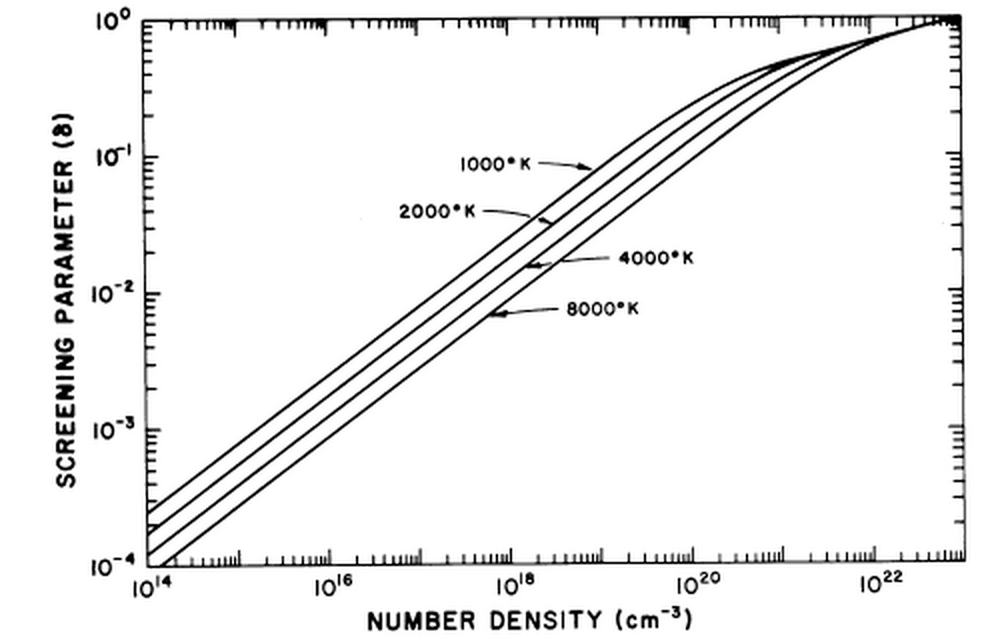
\includegraphics[width=\linewidth]{figs/screeningeffects.png}
\caption{\label{fig:screeninge}From \cite{phelpsbajaj1983}, shows the
screening parameter $\delta$ as a function of electron number density
for various temperatures.}
\end{figure}


\section{Abundance of \h\ Ion in Stellar Atmosphere}
The \h\ abundance depends on several factors: the abundance of H, the
abundance of free electrons (ionized from other species present in the
atmosphere, including H), and the factors that lead to the conversion
of \h\ back to H: photoionization and collisions with other particles.  All
of these factors have some sort of dependence on temperature.

%The solar atmosphere is made up about 70\% by mass of H.  As will be
%shown in what follows, the fraction of H atoms that are taken up in
%\h\ is small, and as is shown in section 7.4 of \cite{boehm1989} the
%fraction of H atoms

%Because the creation of \h\ depends not only on the normal Saha
%equation calculation of relative abundances (in our case,
%$N(H)/N(H^-)$) but also on the presence of free electrons the normal
%Saha equation can be written in the form (\citealt{collins1989})
%\beq
%\label{eq:saha}
%\frac{N(H)}{N(H^-)} = \Phi (T) P_e
%\eeq
%where $P_e$ is the electron pressure (and is hence dependent on the
%ionization states of all species present in the solar atmosphere) and
%$\Phi (T)$ is the normal partion functional form of the Saha
%ionization equation

The abundance of an ionized species can be calculated using the Saha
ionization equation, which is given by
\beq
\label{eq:saha}
\frac{N(X_{i+1})}{N(X_{i})} = \frac{(2\pi m k T)^{1.5}}{n_e h^3}\frac{2g_{i+1}}{g_{i}}e^{-\chi/kT}
\eeq
 where $\chi$ is the energy difference between the two ionization
states, $n_e$ is the number density of electrons, $k$ is the Boltzmann
constant, $h$ is the Planck constant, $T$ is the temperature, $X_i$ is
an atom $X$ in the $i$th ionization state, and $g_i$ is the degeneracy
factor corresponding to the $i$th ionization state.  Specifically
for \h\ we get
\beq
\label{eq:thisone}
\frac{N(H)}{N(H^-)} = \frac{(2\pi m k T)^{1.5}}{n_e h^3}2\frac{1}{2}e^{-0.754\textrm{eV}/kT}.
\eeq
In practice using equation~\ref{eq:saha} is complicated by the fact that
$n_e$ is determined by electrons contributed from all species, not
just the specific atom/ion in question.  It can be calculated by
summing over the number density
of ionized particles multiplied by their degree of ionization (whether
they contribute one electron, two electrons, etc.). This is expressed by
\beq
\label{ref:ne}
n_e = \sum\limits_{X,i}i\times n_{Xi}
\eeq
where $X$ again represents a specific atom and $i$ represents the ionization state
of the atom, thus summing over all possible ions of all atoms.  Since,
as can be seen in equation~\ref{eq:saha} $n_{ij}$ also depends on
$n_e$ we end up with a system of equations that, when rounded out with
equation~\ref{ref:ne}, gives us the same number of equations and
unknowns.  However, values for $n_e$ in the sun have been previously
calculated. I will use the value given in \cite{boehm1989}, as
outlined later on.  

The relative contributions of the elements to the overall electron
density can be calculated without actually knowing the electron
density.  If we know the abundance of an element relative to H we can
define a relative contribution factor $R$ by 
multiplying the abundance by the ionization ratio given in the Saha
equation,
\beq
R_i \equiv B \frac{N(X_{i+1})}{N(X_{i})} \frac{N(X_{i})}{N(H)}
\eeq
where $B$ is a normalization constant.

Table~\ref{tab:electroncontribution} shows the abundance, ionization
potential (abbreviated as ``I.P.''), and relative contribution factor $R$ for the species with
the largest contributions to $n_e$ in the solar atmosphere, in order
of increasing atomic number.
Abundances are taken
from \cite{grevesse1998}\footnote{\cite{grevesse1998} did not have an
abundance quoted for Cs, which, with its low ionization potential of
3.894 eV would make a significant contribution to $n_e$ even in low
abundances. \cite{grevesse1998} did not make it clear whether the
omission was due to lack of measurements or lack of Cs.  Since Cs has
one stable isotope, $^{133}$Cs, we cannot conclude its lack in the
solar atmosphere from radioactive decay alone.}   and are in the form $A_j
= \log N(j)/N(H) + 12.0$ where $j$ represents a specific element.
Ionization potentials are taken from \cite{moore1970} and represent
the ionization potentials for {\it first} ionizations only, since
subsequent ionizations have large enough ionization potentials as to
render their contributions to the overall $n_e$ negligible.  $R$ is
normalized so that, for Na (the atom with the lowest atomic number
that makes a significant contribution) $R=1.0$.  Except for H, only
atoms with $R>0.01$ are included in
table~\ref{tab:electroncontribution}.  Other atoms have
too low of abundances and/or too high of ionization potentials to have a
significant contribution to $n_e$.
\begin{table}[h]
\caption{\label{tab:electroncontribution}Data on Atoms with Largest Contributions to Free Electron Count}
\begin{tabular}{c c c c}
Atom & Relative Abundance $A_j$ & I.P. (eV)& $R$\\
H & 12.0 & 13.598 & $\sim$10$^{-5}$\\
%Li & 1.10 & 5.392 & 0.0032\\
Na & 6.33 & 5.139 & 1.0 \\
Mg & 8.151 & 7.046 & 0.54\\
Al & 6.47 & 5.986 & 0.070\\
K  & 5.12 & 4.341 & 1.5\\
Ca & 6.36 & 6.113 & 0.58\\
Rb & 2.60 & 4.177 & 0.17\\
Sr & 2.97 & 5.695 & 0.045\\
Ba & 2.13 & 5.212 & 0.052\\
\end{tabular}
\end{table}

The largest contributions to $n_e$ are made by the alkali metals Na
and K, followed by their same period alkaline earth metal counterparts,
Mg and Ca  (Li and Be have abundances much too low to make
significant contributions to $n_e$).  Rb, the next period alkali
metal, is next in contribution importance, followed by Al, Ba, and
Sr.  Thus, the alkali and alkaline earth metals, with their small
ionization potentials and (in the case of the period 3 and 4 elements)
large abundances, dominate the contributions to $n_e$.  H, the most
abundant atom in the solar atmosphere, only has a contribution
relative to that of Na of one part in $10^5$.  He has a contribution
relative to that of Na of one part in $10^{15}$.  Thus the presence of
alkali and alkaline earth metals in the solar atmosphere provide a
vital contribution to $n_e$ that H and He by themselves cannot make.


\cite{boehm1989} actually cites the electron abundance in terms of the electron
pressure, $P_e=n_e kT$. She
expresses the Saha equation in the logarithmic form
%\begin{align}
\begin{multline}
\log \frac{N(X_{i+1})}{N(X_i)} = \log \frac{u_{i+1}}{u_i}+\log 2 +\\
 2.5 \log T - \chi \theta - \log P_e - 0.48
\end{multline}
%\end{align}
where log is log$_{10}$, $\theta$ is a temperature parameter given by
$\theta = 5040/T$ ($T$ is in Kelvin), and $u$ is the partition function
\beq
u_i = g_i + \sum\limits_{n=2}^{\infty} g_{in} e^{\chi_{in}/kT}
\eeq
which is summed over all the energy levels of a particular species.
Using the value given in \cite{boehm1989} for the electron pressure in
the solar photosphere 
($\log P_e = 1.5$) we can calculate the abundance of \h\ relative to H
(using 5778 K\footnote{From NASA: www.nssdc.gsfc.nasa.gov/planetary/factsheet/ sunfact.html} as $T$)
\begin{multline}
\log \frac{N(H)}{N(H^-)} = \log \frac{4}{1} + \log 2 + 9.40 - 0.658  -
1.5 - 0.48\\ = 7.7
\end{multline}
Inverting we find 
\beq
\label{eq:hminusab}
\frac{N(H^-)}{N(H)}=10^{-7.7} \approxeq 2 \times 10^{-8}.
\eeq
There is only a small fraction of H at any given time in the
photosphere that has become \h.  To understand better why \h\ in such
small abundances has such a large impact on the opacity in visible
wavelengths we must compare its abundance to other species that have
continuum opacities at visible wavelengths.  The Paschen continuum of
hydrogen (ionization from $n=3$) is the only other thing that can contribute
to continuum opacity in the visual spectral range
(\citealt{boehm1989}).  
%\cite{boehm1989} then calculates the relative
%abundances of H($n=e$) to \h\ and finds
We can calculate the relative abundance of H($n=3$) to \h.
\beq
 \frac{N(H_{n=3})}{N(H^-)} = \frac{N(H_{n=3})}{N(H_{n=1})}\frac{N(H_{n=1})}{N(H^-)}
\eeq
We can make the approximation that $N(H_{n=1})\approxeq N(H)$ since (as will be shown over the course of the next several equations) the number of H atoms with electrons in an excited state is small.
\beq
 \frac{N(H_{n=3})}{N(H^-)} = \frac{N(H_{n=3})}{N(H_{n=1})}\frac{N(H)}{N(H^-)}
\eeq
\cite{boehm1989} calculates the number of H atoms with electrons excited to $n=3$ relative to H atoms in the ground state and gets
\beq
\frac{N(H_{n=3})}{N(H_{n=1})} \approxeq 6 \times 10 ^{-10}.
\eeq
For consistency the value calculated by \cite{boehm1989} for
$N(H)/N(H^-)$ will be used, since she used a slightly different temperature than I did in my calculation (equation~\ref{eq:hminusab}) for consistency.  She calculated $N(H)/N(H^-) \approx 3 \times 10^{-8}$.  Plugging in the values we get
\beq
\frac{N(H_{n=3})}{N(H^-)} \approxeq \frac{6 \times 10 ^{-10}}{3 \times 10^{-8}} = 2 \times 10^{-2}.
\eeq
So, there is about 100 times more \h\ than hydrogen atoms at $n=3$;
assuming that the absorption coefficients of \h\ and  hydrogen atoms
at $n=3$ are within a factor of 10 it can be clearly seen from this
calculation alone that \h\ will be the dominating contribution to the
opacity at visual wavelengths.

%The Balmer continuum is in UV
\cite{boehm1989} also shows that \h\ is only about 10 times less abundant than hydrogen atoms in $n=2$.  Since the Balmer ionization energy (corresponding to photon wavelength of 3647 \AA) occurs in the ultraviolet, where \h\ contributions to opacity are less than in the optical, and there is a relatively large fraction of H$_{n=2}$ relative to \h\ there is a measurable increase in continuum opacity due to H$_{n=2}$.  %Indeed, figure~\ref{fig:bohmopacity} shows the Balmer discontinuity in the ultraviolet.



\section{The Contribution of \h\ to Stellar Opacities}
\subsection{Opacity Due to Bound-Free Absorption}
Bound-free \h\ is the dominant contribution to opacity in the solar atmosphere for photons in the infrared (with wavelength $\lambda \gtrsim 1.6 \mu$m), optical, and ultraviolet regimes; since the solar luminosity peaks in this wavelength range \h\ opacity affects a significant portion of the light coming from the sun.

\cite{wishart1979} calculates the bound-free photoionization
cross-section of \h\ using close-coupling plus correlation
wavefunctions as a function of photon
over the wavelength range 1250-16300 $\AA$.  The cross-sections given
in that reference are accurate to within 1\%.
The calculated cross sections are shown as the points in
figure~\ref{fig:bfcrosssection}; the lines connecting the points are a
cubic spline interpolation.  The right side of the figure shows the
cross-section for photons with energies close to the $0.75$ eV
sufficient to ``ionize'' the \h ion to become H.  The cross-section
peaks at $\sim 8500$\AA and then decreases with increasing photon
energy.  It is interesting to note that this cross-section peaks in
the optical with large values in the near infrared and near
ultraviolet, just as does solar spectrum.  Hence, the \h\ opacity is
most relevant is the regime of photon energies where the sun's own
photon production peaks.  This coincidence causes the \h\ opacity to
be even more dominant in the sun than in stars with a similar \h\
density in their atmospheres but with a photon energy spectrum peaking
outside the optical.
\begin{figure*}{h}
\includegraphics[width=150mm]{figs/boundfree_crosssection.pdf}
\caption{\label{fig:bfcrosssection}The bound-free photoionization
cross-section of \h. Tabulated values calculated
by \cite{wishart1979} are given as open circles with a cubic spline
interpolation shown as the line connecting the points.  The calculated
cross-sections span from near infrared (at the wavelengths where photon
energies are sufficiently high to ionize the least bound electron
of \h) to near ultraviolet. As shown, photon energy increases along
the x-axis from right to left.}
\end{figure*}

Figure~\ref{fig:bohmopacity} shows  opacity as a function of wavelength over the range of wavelengths where \h\ bound-free opacities are relevant for a theoretical solar-like star.  At high wavelengths, past the $\sim 1.6 \mu$m cutoff for \h\ opacity free-free interactions with \h\ dominate the opacity (the H in the figure is a typo, it should be \h), while at lower wavelengths Balmer bound-free absorption begins to dominate the opacity.
\begin{figure}{h}
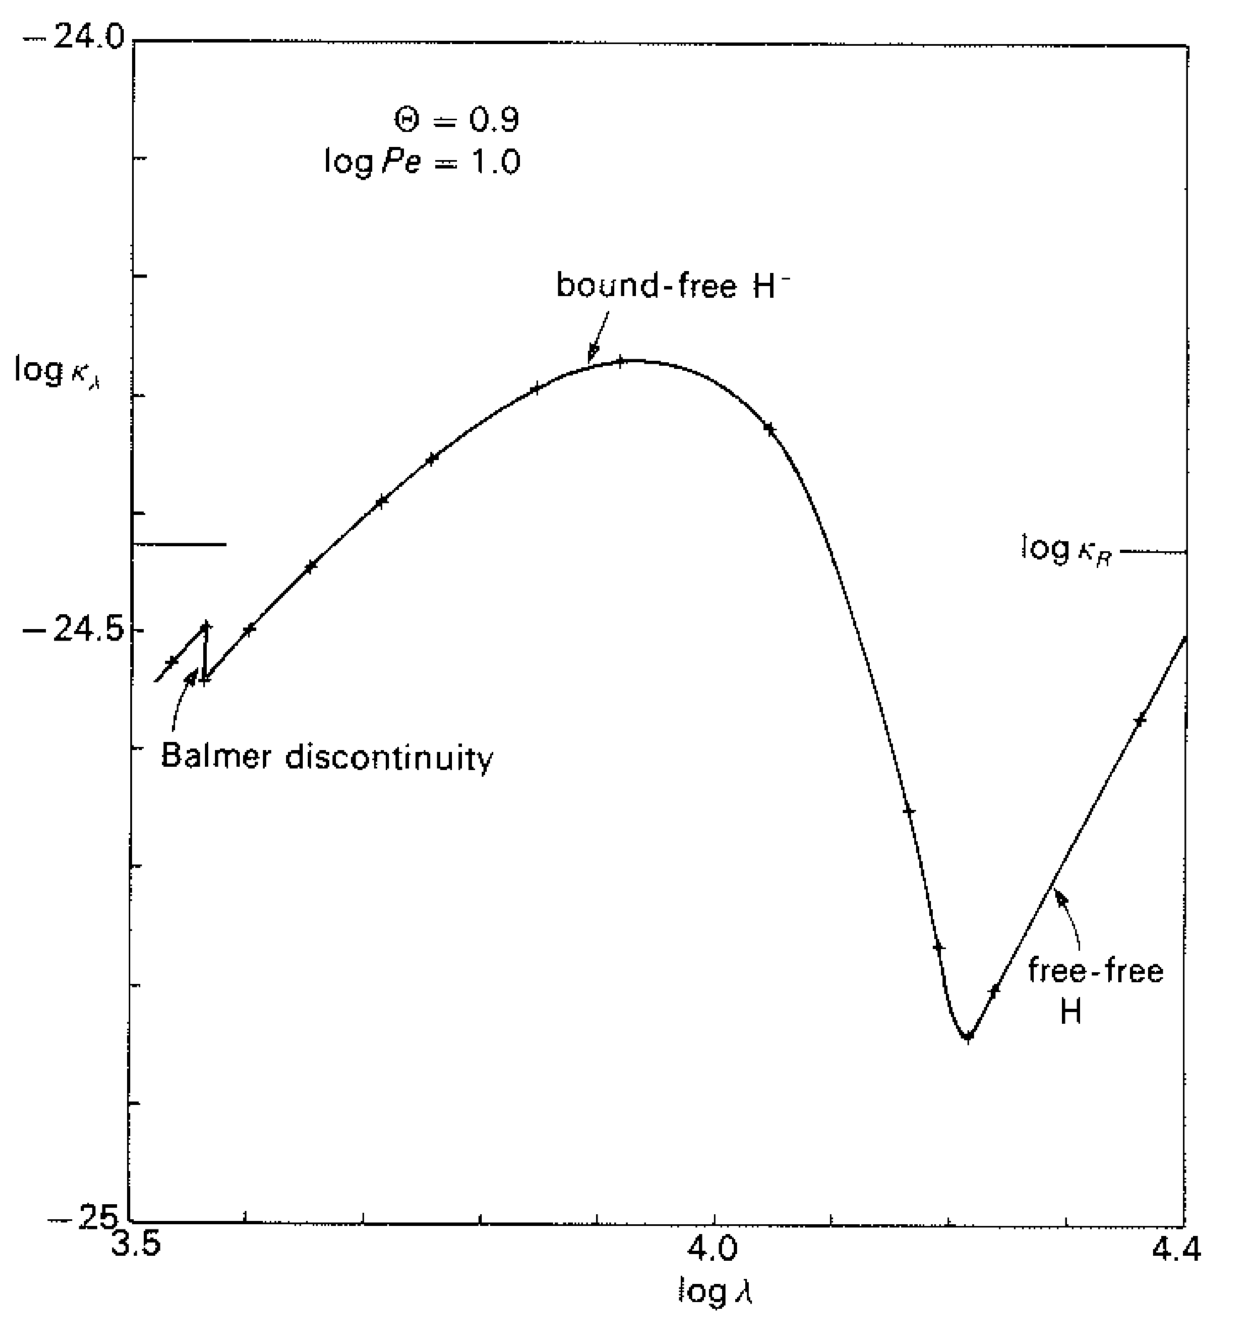
\includegraphics[width=80mm]{figs/hminusopacity.png}
\caption{\label{fig:bohmopacity}Continuous absorption coefficient per heavy particle, shown for $\Theta=0.9$ (which means $T=5600$ K and log $P_e=1.0$.  Note that the free-free contribution is mislabelled; it should be free-free from \h\ not H.  Figure from \cite{boehm1989}.}
\end{figure}

Figures~\ref{fig:bfcrosssection} and \ref{fig:bohmopacity} both show that the opacity doesn't show a discontinuity at the $\sim$1.6$\mu$m cutoff value for \h\ ``ionization'' as would be expected and is indeed seen for other species being ionized.  Figure~\ref{fig:bethe} (taken from \citealt{bethe1977}) shows $\sigma$ as a function of photon frequency relative to the frequency corresponding to the ionization energy $\nu$ for H, He, and \h.  H and He both show a large cross-section right at the threshold frequency which decays with increasing frequency; \h, however, shows a small cross-section right at the threshold which increases and reaches a maximum at $\nu/\nu{thr}\sim$1.7.  \cite{rau1996} explains this in terms of basic quantum mechanics and angular momentum.  After a photon is absorbed by \h\ the electron departs in a $p$-wave.  In the ground state of \h, however, both the electrons are in the $s$ orbital.  Thus there is an angular momentum barrier that must be overcome, via quantum tunnelling.  Just above the ionization threshold electrons have low energy and see the angular momentum barrier as the longest range potential; the probabilities associated with tunnelling through this barrier thus affect the cross-section at these low energies. .  {\bf Can talk about Wigner 1948 E to the l+1/2 if you want. Rau page 116}.  This is not the case for neutral atoms, where the Coulomb potential is the longest-range potential.  This potential has no dependence on angular momentum and, as such, there is no angular dependence on the cross-section.
\begin{figure}{h}
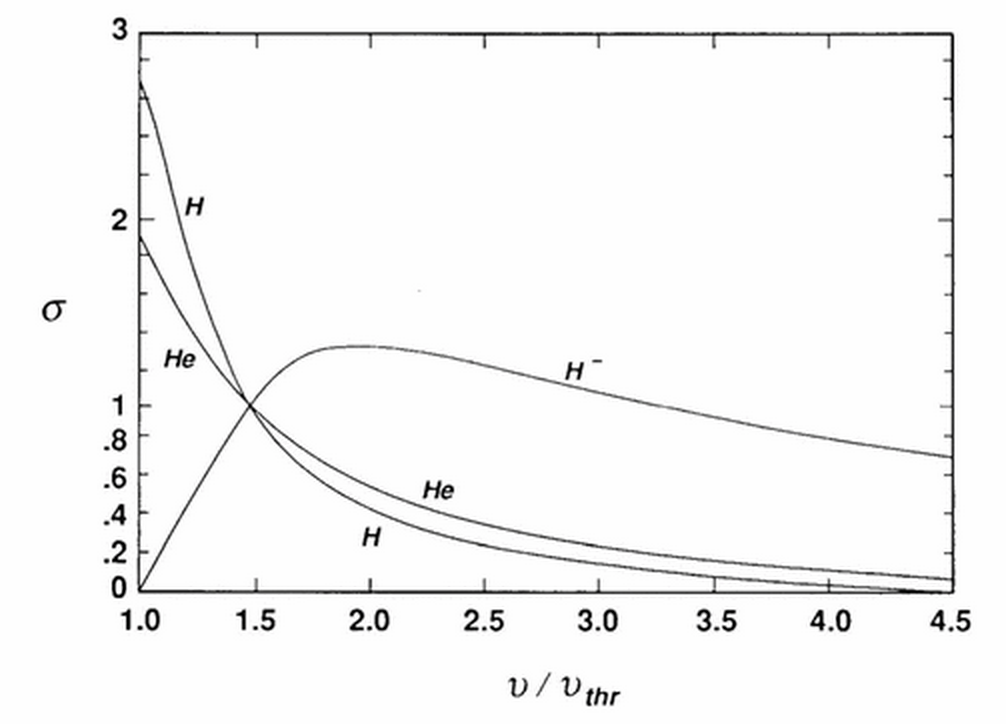
\includegraphics[width=80mm]{figs/betheplot.png}
\caption{\label{fig:bethe}Photoionization cross-section as a function of photon frequency, expressed in the unitless ratio $\nu/\nu_{thr}$, which is the ratio of the photon frequency relative to frequency of a photon with energy corresponding to the ionization energy of the species.  Cross-sectionsH, He, and \h\ are shown (from \citealt{bethe1977}).}
\end{figure}

\subsection{Opacity Due to Bound-Free Absorption}
At wavelengths greater than $\sim1.6\nu$m free-free absorption on \h\ provides a significant contribution to the opacity.  Free-free absorption, also known as inverse Bremstrahlung absorption, is the process by which an electron absorbs a photon in the presence of an electric field provided by an atom or ion.  For \h\ the process looks like
\beq
\gamma + e^- + H^- \rightarrow e^- + H^-.
\eeq
\cite{bell1987} calculate the absorption coefficient for free-free absorption on \h\ for various temperatures.  They include s $\leftrightarrow$ p and p $\leftrightarrow$ d transition contributions only, saying that contributions from higher partial waves are negligible.  They use the notation $\theta=5040 K /T$. Their calculations are shown in table~\ref{tab:freefreetable}.  It is worth noting that the free-free absorption coefficient increases with increasing wavelength, allowing it to contribute significantly to the opacity at wavelengths longer than the $\sim 1.6\nu$m cutoff for \h\ bound-free absorption.  The absorption coefficient also increases with decreasing temperature (represented by increasing $\theta$).  For reference purposes,  the sun has $\theta=0.87$.
\begin{table}
\caption{\label{tab:freefreetable}\h\ free-free absorption coefficient as calculated by \cite{bell1987}}
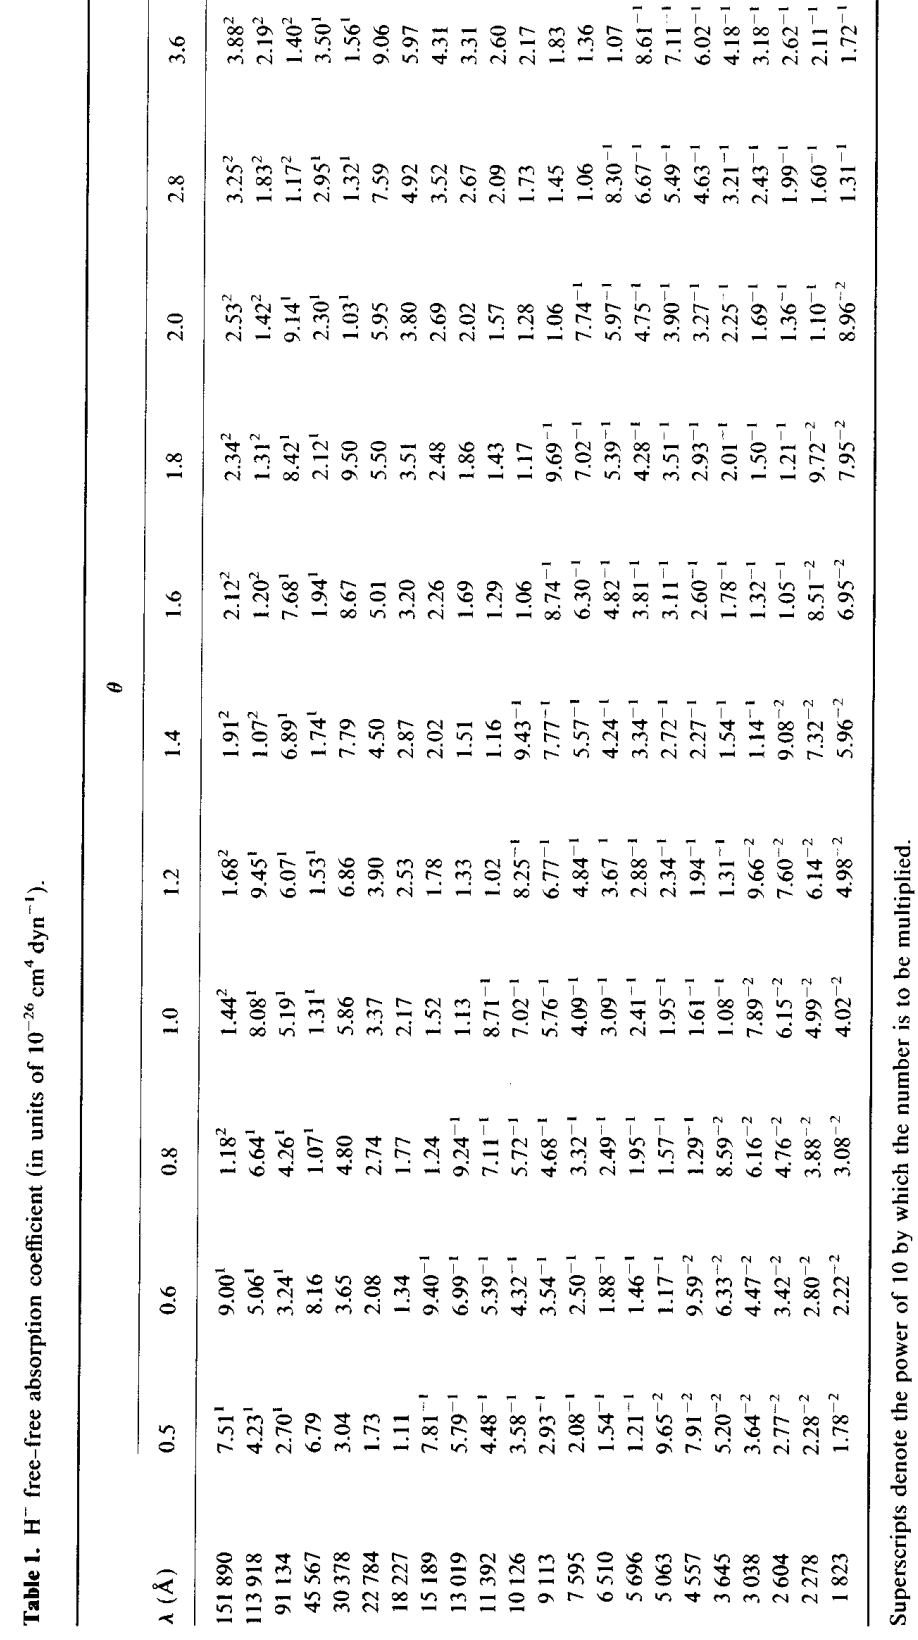
\includegraphics[width=\linewidth]{figs/freefreetable.png}
\end{table}

This brings up the question about how the absorption coefficient contribution from \h\ changes at $\sim 1.6 \mu$m, where bound-free absorption becomes relevant.  Table~\ref{tab:boundfreecomp}, taken from \cite{bell1975} provides a partial answer.  Please note in table~\ref{tab:boundfreecomp} that the top line beginning with $\lambda$ should read ``$\lambda(\AA)\theta=$''. The $\theta$ is not clear in the grainy rendition of the table.  This is the same $\theta$ as in table~\ref{tab:freefreetable}.  Moving from 18225 \AA\ to 15188 \AA, over the wavelength range where bound-free absorption starts to become relevant, the coefficient for $\theta=$0.8 decreases\footnote{Although the exact nature of the decrease for $\theta=$0.8 is hidden in the low wavelength resolution of the table, over the range of $\sim$300 \AA between 18225 \AA\ to 15188 \AA\ the coefficient may reach a minimum and start to increase again and still produce the numbers we see in table~\ref{tab:boundfreecomp}.} while for the other $\theta$ it increases, although in some cases only modestly. Larger $\theta$, corresponding to lower temperature, produce a larger increase in the absorption coefficient in this range.  The modest increase at higher temperatures may seem puzzling at first but a quick review of figure~\ref{fig:bethe} reminds us that the bound-free absorption cross-section for \h\ does not exhibit a sudden jump at the cutoff wavelength as would be seen for other species undergoing photoionization, but rather increases fairly modestly, reaching a maximum only for wavelengths less than the cutoff wavelength.  For the next tabulated value of wavelength, $\lambda=11391$\AA, all absorption coefficients are shown to be increasing.  This table reflects the somewhat gradual transition from \h\ free-free absorption to \h\ bound-free absorption as being the dominant contribution of \h\ to the opacity, as can be seen in figure~\ref{fig:bohmopacity}, in contrast with the sudden increase in opacity from Balmer bound-free absorption seen in the same figure.
\begin{table}
\caption{\label{tab:boundfreecomp}\h\ total absorption coefficient as calculated by \cite{bell1975}}
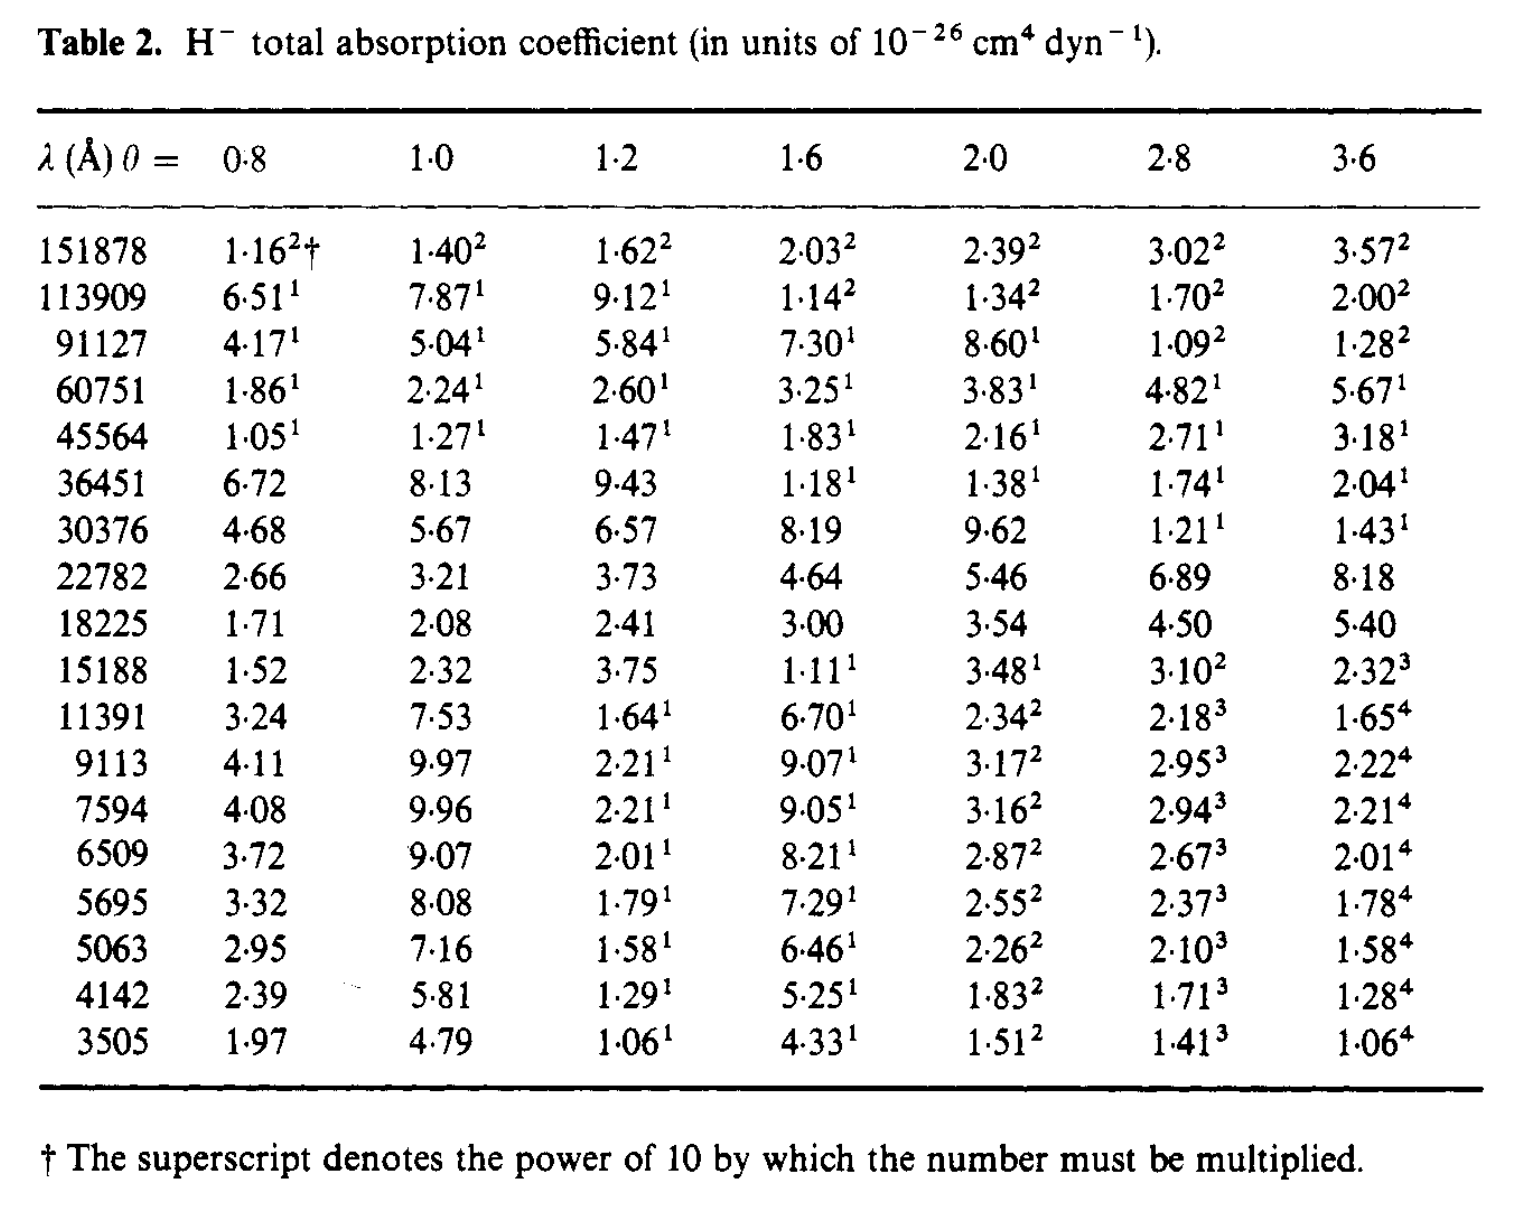
\includegraphics[width=\linewidth]{figs/freeandboundtable.png}
\end{table}

It would be nice to compare directly the values of table~\ref{tab:freefreetable} with those used to generate figure~\ref{fig:bfcrosssection} but they are in different units so direct comparison is not possible as is.  However, \cite{chandra1946} provide an early theoretical calculation of the total absorption coefficient due to both free-free and bound-free absorptions for \h, shown in figure~\ref{fig:chandratotal}.  In this figure the total absorption coefficient has a local minimum around $\sim1.65\mu$m, close to the cutoff wavelength for \h\ bound-free absorption (at $T$=6300 K).  Thus, although the bound-free contribution is smaller than the free-free contribution around the cutoff wavelength, it immediately begins to have a significant effect on the total absorption coefficient, at $T$=6300 K at least.  Figure~\ref{fig:bohmopacity} shows a minimum somewhere between $\sim$14000-16000\AA\ for her calculation of the opacity at $T$=5600 K and $P_e=1.0$.  She also makes the comment that the sum of the free-free and bound-free contributions to the opacity has a minimum between $\sim$16000-16500\AA. Thus it appears that, in the sun, the bound-free contribution to the absorption coefficient becomes significant either right at or within a few hundred \AA ngstrom of the cutoff wavelength.
\begin{figure}
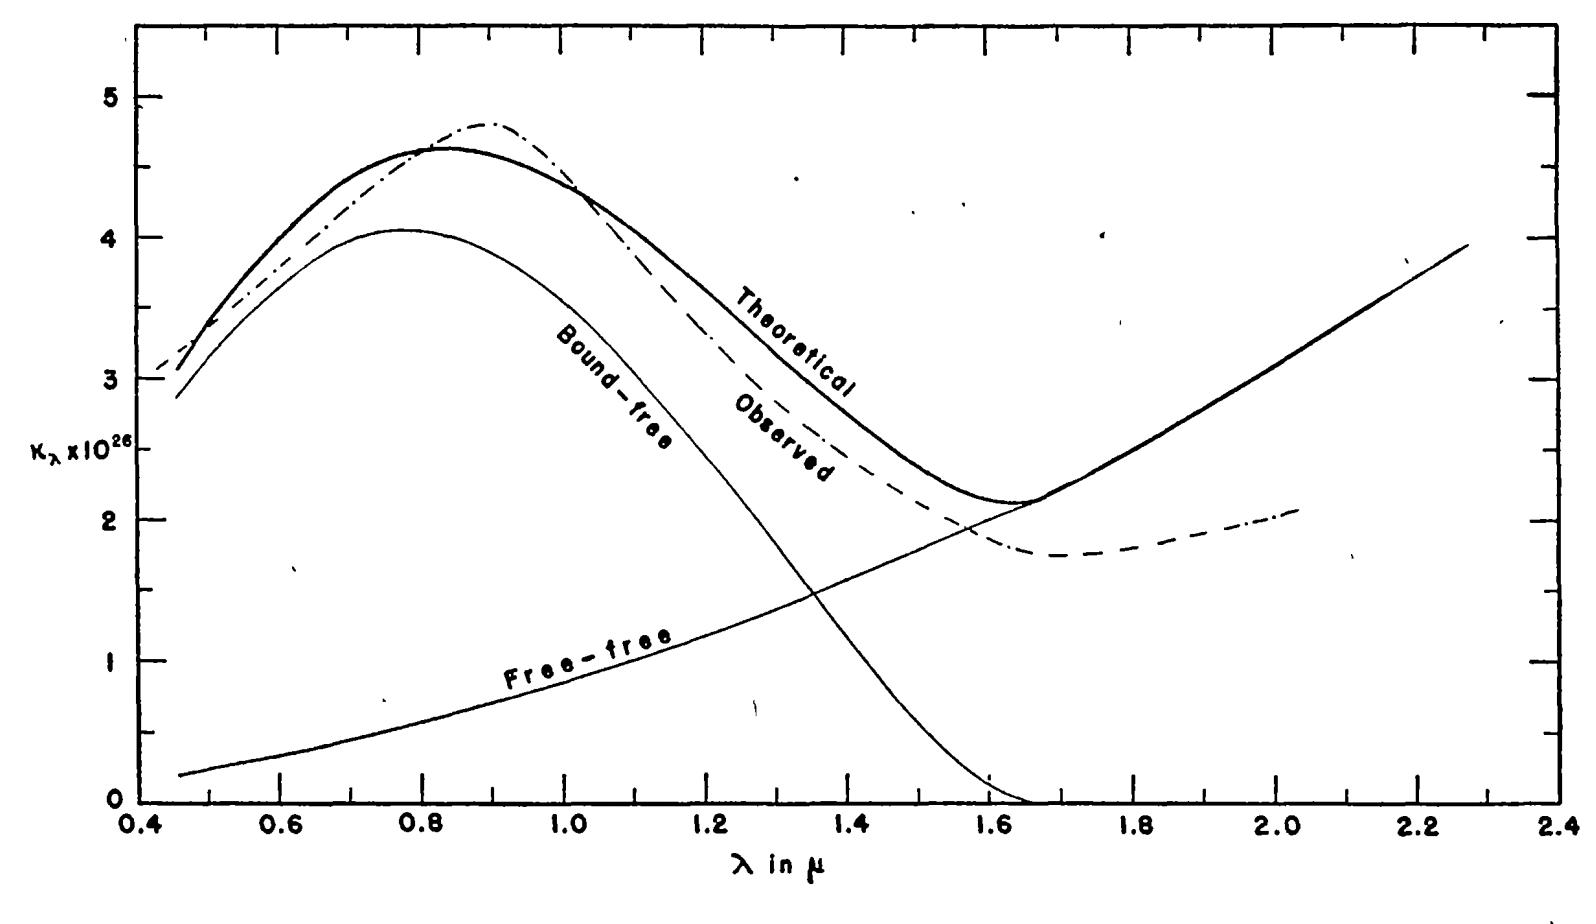
\includegraphics[width=\linewidth]{figs/chandraopacity.png}
\caption{\label{fig:chandratotal}From \cite{chandra1946}, the continuous absorption coefficient of \h\ per neutral hydrogen atom per unit electron pressure for a temperature of 6300 K.  A comparison with the observed values is made, shown with the dotted line.  The curve marked ``theoretical'' represents the sum of the free-free and bound-free curves.}
%M&B and W&W correspond to earlier determinations of the same quantities, by Massey and Bates (bound-free) and  \cite{wheeler1942} (free-free) respectively. No further reference to Massey and Bates other than their names could be found in \cite{chandra1946}.
\end{figure}

Plunk in somewhere: free-free
\begin{equation}
\kappa = \frac{3.7062}{k(k^2+0.05512)}\left\lvert \int_0^{infty}W)x(r)\chi_1(r)dr \right\rvert^2 \times 10^{-18} \textrm{cm}^2
\end{equation}
where $k$ is the momentum of the ejected electron in atomic units, $W_2(r)$ is a certain weight function which can be tabulated (values are shown in \citealt{chandra1945}, and $\chi_1(r)$ is the radial part of a p-spherical wave in the Hartree field of a hydrogen atom which tends ot unit amplitude at infinity (\citealt{chandra1945}).


\section{Stellar Environments where \h\ Opacities are Dominant}
Talk about both the fact that there needs to be \h\ and also how in
some stars the Paschen, other series start to be relevant.

\section{\h\ in a General Astrophysical Context}
The 1.6$\mu$m bump is an astrophysical feature detected in extragalactic settings.  Because of the minimum of \h\ opacity around 1.6$\mu$m which causes a maximum in the observed spectral energy distributions (SEDs) of cool stars (\citealt{sawicki2002}) which feature can be detected in the integrated light from all stars in a galaxy.  For galaxies with $z\sim1$ this feature will fall into {\it Spiter}'s 3-8 $\mu$m IRAC bands.  \cite{desai2009} claim that the rest-frame 1.6$\mu$m bump can be used to select highly obscured star forming galaxies at $z\approx 2$.  %They also state that galaxies detected

\h\ ions are also important in the gas-phase formation of H$_2$ in the
interstellar medium (ISM).  The associative detachment reaction is (\citealt{draine2010})
\beq
H^- + H \rightarrow H_2 + e^- + \textrm{KE}.
\eeq
However, \h\ can also be destroyed in the ISM by interaction with
other positive ions
\beq
H^- + X^+ \rightarrow H + X
\eeq
where $X$, as before, stands for any atomic species.


%\section{ISM \h\, our hope to detect it}

\bibliographystyle{apj}
\bibliography{bibliography}


\end{document}
